\documentclass[a4paper, 12pt, titlepage]{article}
\usepackage{graphicx}
\usepackage{titlesec}
\usepackage{hyperref}
\graphicspath{{Images/}}
\setcounter{secnumdepth}{4}
\hypersetup{
	colorlinks=true,
	linkcolor=black,
	filecolor=magenta,      
	urlcolor=cyan,
}
%opening
\title{
	\begin{figure}[h]
		\centering
		
\includegraphics{polimi_logo}
	\end{figure}
	Politecnico di Milano, A.A. 2016/2017 
	\newline\newline 
	Software Engineering 2: PowerEnJoy 
	\textbf{R}equirements \textbf{A}nalysis and \textbf{S}pecification \textbf{D}ocument}
\author{Binosi Lorenzo 876022}
	
	
\begin{document}
	
	\maketitle
	\tableofcontents
	\newpage
	
	\section{Introduction} \label{sec introduction}


\subsection{Purpose}

The Design Document has the purpose to provide a functional description of the system. It defines the design of the software architecture, its components and their interactions, provided with the used algorithms and the user interfaces design. 

The document is written for project managers, developers, testers and quality assurance. It can be used for a structural overview to help maintenance and further development.


\subsection{Scope}

PowerEnJoy is a large-scale car-sharing service. It requires to perform excellently, to be secure, easily modifiable and as available as possible. Minding these necessities, in the following chapters will be shown how the system is structured and and which were the reasons that led to such decisions.
  
\subsection{Definitions, Acronyms, Abbreviations}

\begin{description}
	\item[DD:] Design Document.
	\item[RASD:] Requirements Analysis and Specification Document.
	\item[System:] the whole software system to be developed, comprehensive of all its parts.
	\item[REST:] REpresentational State Transfer. It's an architectural style and an approach to stateless communications, used in the development of client-server systems.
	\item[GUI:] Graphical User Interface.
	\item[ACID:] Atomicity, Consistency, Isolation, Durability. A set of properties of database transactions.
	\item[API:] Application Programming Interface.
	\item[EJB:] Enterprise Java Bean.
	\item[JPA:] Java Persistence API.
	\item[JSP:] JavaServer Pages.
	\item[HTTP:] HyperText Transfer Protocol.
	\item[HTTPS:] HyperText Transfer Protocol Secure.
\end{description}

\subsection{Reference Documents}

This document refers to the project rules of the Software Engineering 2 project~\cite{se-project-rules} and to the DD assignment~\cite{se-assignment}.

\subsection{Document Structure}

This document is structured in five parts:
\begin{description}
	\item[\autoref{sec introduction}: Introduction.] This section provides general information about the DD document and the used terms.
	\item[\autoref{sec architectural design}: Architectural Design.] This section shows the software architecture of the system, with its components and their interactions.
	\item[\autoref{sec algorithm design}: Algorithm Design.] This section will present and discuss in detail the algorithms designed for the system functionalities, independently from their concrete implementation.
	\item[\autoref{sec user interface design}: User Interface Design.] This section shows how the user interface will look like and behave, by means of concept graphics and UX modeling.
	\item[\autoref{sec requirements traceability}: Requirements Traceability.] shows how the requirements in the RASD~\cite{rasd} are satisfied by the design choices of the DD.
\end{description}
	
	\section{Overall Description}\label{sec overall-desc}

\subsection{Product Perspective}
PowerEnJoy system is a simple client-server architecture based on a back-end server application and diffent front-end client applications, supported by different operating systems.

\subsubsection{User Interfaces}
Guests and users can interact with the service via the web application or the mobile application. Drivers can find other service functionalities in the car application. It is necessary to provide a common and uniform look and feel among the different hardware architectures.

All interfaces shall be intuitive and user friendly. They should not require the reading of detailed documentation to be used.

\subsubsection{Hardware Interfaces}

All cars are provided with a dedicated embedded system connected to several plugins and a touchscreen display used for interact with the car application.
Thanks to this embedded architecture the system will also be notified about the status of the car and its location, even if the main battery is completely discharged.

\subsubsection{Software Interfaces}

Mobile application and web application are supposed to be friendly with any device, in particular the first one must be developed for iOS and Android, and the second one will work on any operating system that support a web browser.

On the embedded system of any cars is installed a JVM that runs a Java application that provides informations to the driver and to the system.

The back-end server stores its data in a RDBMS and can run on every platform that supports the JVM. It also provides different APIs for different functions that a user, or a guest, can do through client applications. 

\subsection{Product Functions}
\begin{figure}[H]
	\centering
	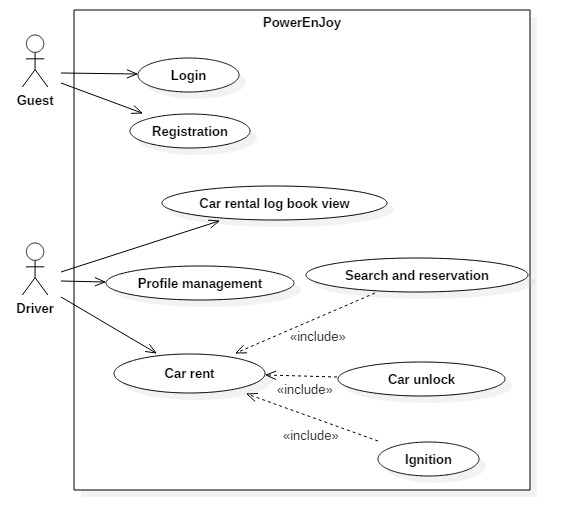
\includegraphics[width=\textwidth]{use_cases/PowerEnJoy.jpg}
	\caption{The comprehensive use-case diagram of all the functionalities implemented by the system.}
\end{figure}

\begin{figure}[H]
	\centering
	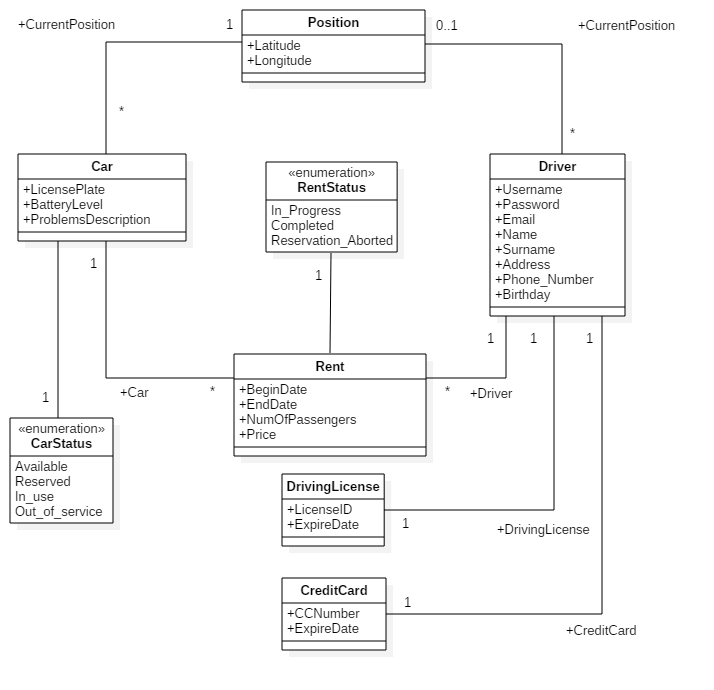
\includegraphics[width=\textwidth]{uml/PowerEnJoy.jpg}
	\caption{The comprehensive class diagram of the system.}
\end{figure}

The following lists reassume what anyone can do interacting with the system.
\begin{itemize}
	\item Guests can:
	\begin{itemize}
		\item create an account (sign up to the system)
		\item log in
	\end{itemize}
	\item Drivers can:
	\begin{itemize}
		\item edit profile informations
		\item delete their account
		\item rent a car
		\item access to the car rental log book
	\end{itemize}
\end{itemize}

\subsection{User Characteristics}

The only users of the system are drivers. Drivers must provide a valid driving license and a valid payment method in order to register to the service.

It's granted that drivers have access to an internet connection.

\subsection{Constraints}

\subsubsection{Regulatory policies}
Any driver must follow current traffic and regulamentation laws of the area where the system is operating its car-sharing service. Driving licenses from other countries must be compatible with the laws of the country where the service is operating.

The system must ask the driver for the permission to acquire, store and process personal data and web cookies.

\subsubsection{Interfaces to other services}

PowerEnJoy needs to communicate with a service to solve all those issues that can hit a car or that can happen while using it. These problems may be:
\begin{itemize}
	\item breaking of one or more parts of the car
	\item battery power lower than 25\%
	\item accidents
	\item faulty communication between system and car
\end{itemize}
The service assigned to this kind of problems, receives all reports that fall in the previously specified cases, and solves them as soon as possible, reporting the results back to PowerEnJoy.

\subsubsection{Hardware limitations}
The service requires an Internet connection fast enough to guarantee a fast response from the server and hardware architectures that can run properly the client side applications (web and mobile apps).

\subsubsection{Reliability requirements}
The system must have a minimum availability of 99\%.

\subsubsection{Parallel operations}
The system must support parallel operations from different drivers that may require access to the database.

\subsection{Assumptions and Dependencies}

It's assumes that:
\begin{itemize}
	\item All drivers have access to a stable internet connection.
	\item All cars are the same model, so that any of them will have the same number of seats
	\item The number of cars is sufficient to satisfy the demand in each area.
	\item All the areas where the system is operating are covered by a reliable 3G/4G connection.
	\item The system is operating in an area composed by a city or agglomerated cities, of the same country, closed each other.
\end{itemize}

\subsection{Future Extensions}
The system will be implemented foreseeing the possibility of further extensions, for example:

\begin{enumerate}
	\item If a car is left at special parking areas where they can be recharged and the driver take care of pluggin the car into the power grid, the system applies a discount of 30\% on the last ride.
	\item If a car is left at more than 3 KM from the nearest power grid station or with more than 80\% of the battery empty, the system charges 30\% more on the last ride to compensate to compensate for the cost required to re-charge the car on-site.
	\item If the driver enables the money saving option, he/she can input his/her final destination and the system provides informations about the station where to leave the car to get a discount. This station is determinate to ensure a uniform distribution of cars in the city and depends both on the destination of the driver and on the availability of power plugs at the selected station.
\end{enumerate}
	
	\section{Specific Requirements}\label{sec requirements}

\subsection{External Interface Requirements}

\subsubsection{User interfaces}

User interfaces must satisfy the following UI constraints:
\begin{itemize}
	\item Web application
	\begin{enumerate}
		\item Web pages must adhere to the W3C standards. In particular, the software shall conform to the HTML~5~\cite{w3c-html5}, CSS~\cite{w3c-css} standards.
	\end{enumerate}
	\item Mobile application
	\begin{enumerate}
		\item The iOS version must adhere to the iOS Human Interface Guidelines~\cite{apple-ios-hig}.
		\item The Android version must follow Android design guidelines~\cite{google-android-hig}.
	\end{enumerate}
		\item Common to web and mobile applications:
		\begin{enumerate}
			\item The client applications must have an UI that is accessible to disabled people.
			\item The interface must offer the possibility to choose the language used at all times.
			\item The first screen (homepage) must ask the guest to log in or sign up in order to begin operations.
			\item Once logged, the homepage must show the car search page. It also includes one button for log out and buttons that open different pages. These pages are:
				\begin{itemize}
					\item reservation page; where the driver can find the functionality in order to unlock the car. The page also provides informations about the reserved car.
					\item profile management page; where the driver can manage his/her profile informations or update his/her driving license and payment method.
					\item car rental log book page; where the driver can find information about his/her past rentals.
				\end{itemize}
			\item UI controls and views must be suitable for the input interface and the screen size.
		\end{enumerate}
	\item Car application
	\begin{enumerate}
		\item radio and GPS navigator applications must be implemented.
		\item always notifies the driver about his/her current charges.
	\end{enumerate}
	\item Server back-end
	\begin{enumerate}
		\item The server back-end must be configurable by means of a configuration text file.
	\end{enumerate}
	
\subsubsection{Hardware interfaces}
The embedded system of any cars must be provided of	
\begin{itemize}
	\item a 7" touchscreen display
	\item a GPS device
	\item sensors that check if all the parts of the car are working correctly
	\item sensors that check how many passengers are on the car
	\item a 4G router for a stable Internet connection
	\item a secondary battery used only if the main battery is discharged. The car can't use this battery
\end{itemize}

\subsubsection{Software interfaces}
The required software products used by the back-end are:
\begin{itemize}
	\item MySQL 5.7\footnote{\url{http://dev.mysql.com}}
	\item Java SE 8\footnote{\url{http://www.oracle.com/technetwork/java/javase/overview/index.html}}
\end{itemize}
The required software product used by the car application is:
\begin{itemize}
	\item Java Embedded\footnote{\url{http://www.oracle.com/technetwork/java/embedded/overview/index.html}}
\end{itemize}
The required operating systems for the mobile application are:
\begin{itemize}
	\item iOS 8 or better
	\item Android 6.0 or better
\end{itemize}

A set of APIs for the several functionalities must be provided by the system
	
\subsubsection{Communications interfaces}
The clients communicate with the server via HTTPS requests (port 443).

\end{itemize}

\subsection{System Features}

\subsubsection{Driver registration}

\subsubsubsection{Purpose}
Any guest can subscribe through web or mobile applications.

In both cases the guest has to fill a registration form and must agree to the personal data policy according to his/her country privacy laws, otherwise the registration request will be aborted.

As soon as the guest has submitted all the data, the system verifies the consistency of the information and a confirmation mail with a password is sent to the email address indicated in the registration form. The guest must confirm his/her email address to end the registration.

Once registered a guest can be recognized as a driver by logging in.

\subsubsubsection{Scenario 1}
Bob, a normal citizen without a car, has just discovered the existence of the PowerEnJoy service and wants to use it.

He opens the homepage of PowerEnJoy website and proceeds to register by clicking on the button "Sign up".

He fills in all the information required and authorises the personal data treatment. 

The system verifies all the information that bob submitted in the form and sends him a confirmation mail.

Bob checks his mailbox, opens the email and clicks on "Confirm email". He is also notified about his current password.

The system then informs Bob that he is successfully registered.

\begin{figure}[H]
	\centering
	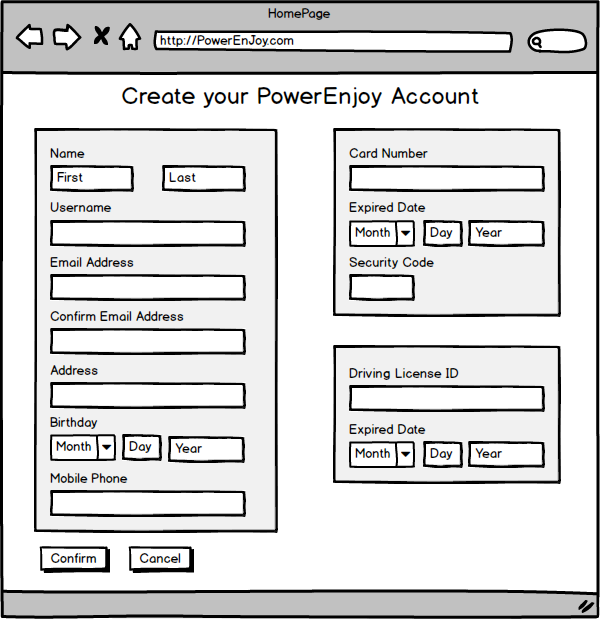
\includegraphics[width=\textwidth]{mockup/WebRegistration.png}
	\caption{Concept for the registration webpage.}
\end{figure}

\begin{figure}[H]
	\centering
	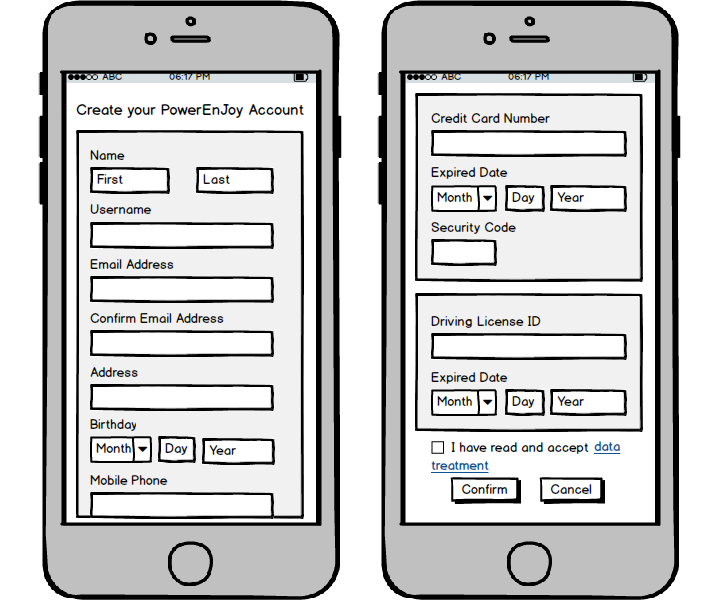
\includegraphics[width=\textwidth]{mockup/MobileRegistration.png}
	\caption{Concept for the mobile registration page.}
\end{figure}

\subsubsubsection{Use case description and sequence diagram}

\begin{table}[H]
\begin{center}
	\begin{tabular}{| l | p{0.6\textwidth} |}
		\hline
		Actor & Guest \\
		\hline
		Goal & G3
		\\
		\hline
		Input condition & The guest chooses to create a new driver account.  \\
		\hline
		Event Flow & \begin{enumerate}
			\item The registration form is loaded and the guest compiles it.
			\item The guest authorizes the personal data treatment.
			\item The guest clicks on "Confirm".
			\item The system sends a confirmation email.
			\item The guest reads the e-mail containing his/her password, received by PowerEnJoy and clicks on the link to confirm the registration.
		\end{enumerate}
		\\
		\hline
		Output condition & The system tells the guest that he/she has been successfully registered. \\
		\hline
		
		Exception &  \begin{itemize}
			\item Some exceptions are handled by notifying the guest of the problem through a dynamic message box or reloading the registration form.
			
			The requirements that generate these kind of exceptions are:
			\ref{f-sameinfo},   %The username/e-mail is already used by someone else.
			\ref{f-samelicense}, %The driving license is already used by someone else.
			\ref{f-usrn},       %The username doesn't respect the restrictions.
			\ref{f-wrongmail},  %The emails are not equals.
			\ref{f-licenseexp}, %The driving license is expire
			\ref{f-cc}.			%The payment method is not valid.
			
			\item Some exceptions are handled aborting the registration (all guest's data are deleted).
			
			The requirements that generate these kind of exceptions are:
			\ref{f-dataTreat},   %The user doesn't authorises the data treatment.
			\ref{f-confirm}.   %The user doesn't confirms the registration clicking on the link received via e-mail.
		\end{itemize}
		\\
		\hline
	\end{tabular}
\end{center}
\end{table}

\begin{figure}[H]
	\begin{center}
		\centering
		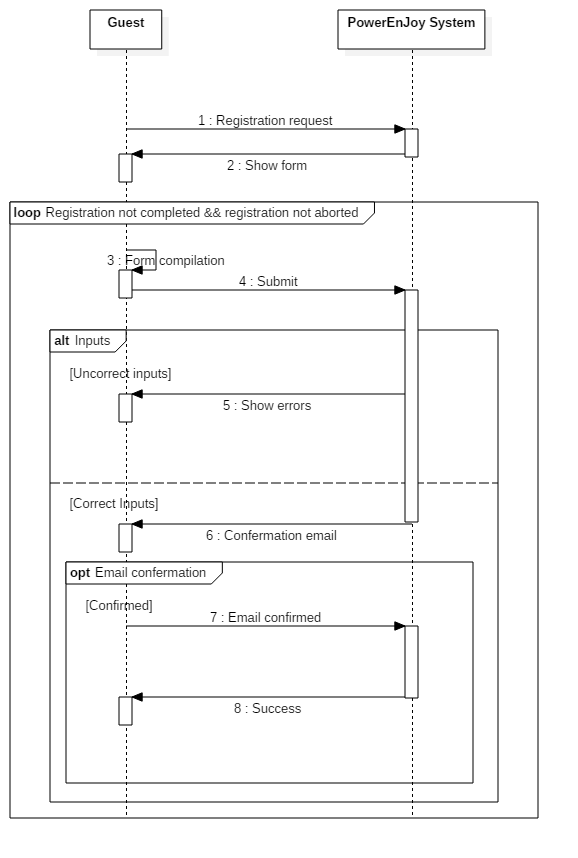
\includegraphics[height=0.9\textheight, keepaspectratio]{sequence_diagram/Registration.jpg}
		\caption{Sequence diagram of the registration process.}
	\end{center}
\end{figure}

\subsubsubsection{Associated functional requirements}

\begin{enumerate}
	\item Guests must provide the following information:
	\begin{itemize}
		\item name
		\item surname
		\item username
		\item email address
		\item address
		\item day of birth
		\item phone number
		\item credit card number
		\item credit card date of expire
		\item credit card security code
		\item driving license ID
		\item driving license date of expire	
	\end{itemize}
	\item There mustn't be another user already subscribed with the same username and/or email. \label{f-sameinfo}
	\item There mustn't be another driver already subscribed with the same driving license. \label{f-samelicense}	
	\item Username must match the regular expression\\``\texttt{[a-zA-Z][a-zA-Z0-9]\{2,20\}}''    \label{f-usrn}
	\item The system accepts the email only if it is entered identically both times.\label{f-wrongmail}
	\item The driving license must be valid and not expired.
	\label{f-licenseexp}
	\item The payment method must be valid and not expired.
	\label{f-cc}
	\item If the personal data treatment is not authorised, the subscription is canceled. \label{f-dataTreat}
	\item The system must allow the guest to abort the registration process at any time.
	\item Email confirmation process:
	\begin{enumerate}
		\item The subscription ends successfully when the guest clicks on the link in the confirmation email. It must contain a password for the new driver.
		\item After one day without an answer, the guest's registration info are deleted and the guest may re-try the registration process.  \label{f-confirm}
	\end{enumerate}
\end{enumerate}

\subsubsection{Search and reservation}

\subsubsubsection{Purpose}
Any logged driver, in possession of a valid driving license and a regular status of payments, can search and reserve a car through the web application or the mobile app.

The system shows a map, of the area nearby him/her, with the available cars represented as colorful markers. There are 3 diffent colors for the markers:
\begin{itemize}
	\item red: 25-50\% of battery charge
	\item yellow: 50-75\% of battery charge
	\item green: 75-100\% of battery charge
\end{itemize}
The driver can also search nearby cars from a given address through a search box on the page.

Once the driver chooses the car he can click on its marker and a new dynamic frame will show more informations about the car and the possibility to reserving it by clicking on the button "Reserve".
The system then notifies the driver that he/she succesfully reserved a car.

Cars with less charge than 25\% of battery charge require assistance to be recharged and the system won't show them as available to the drivers. 


\subsubsubsection{Scenario 1}
Bob logs in the PowerEnJoy application through his web browser. He wants to reserve a car because an important meeting is waiting for him. Once logged, the system redirects him to the homepage that now shows the car search page. Bob realizes there's only a car with a red marker within 1km from him. Bob has to hurry up so he clicks on the red marker and then on the button "Reserve". Bob has succesfully reserved the car and he get redirect to the reservation page.

\subsubsubsection{Scenario 2}
Alice logs in the PowerEnJoy application through his mobile phone. She wants to reserve a car but everytime she clicks on the button "Reserve" of an available car the system shows her a dynamic message box that remember her to solve her pending payments. Once any pending payments is solved she will be able to reserve an available car.

\begin{figure}[H]
	\centering
	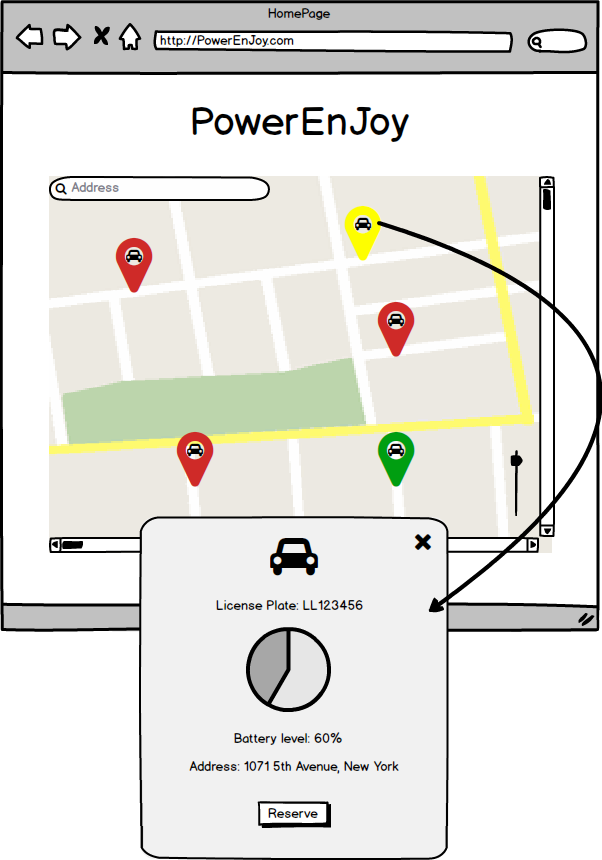
\includegraphics[width=\textwidth]{mockup/WebSearch.png}
	\caption{Concept for the search webpage.}
\end{figure}

\begin{figure}[H]
	\centering
	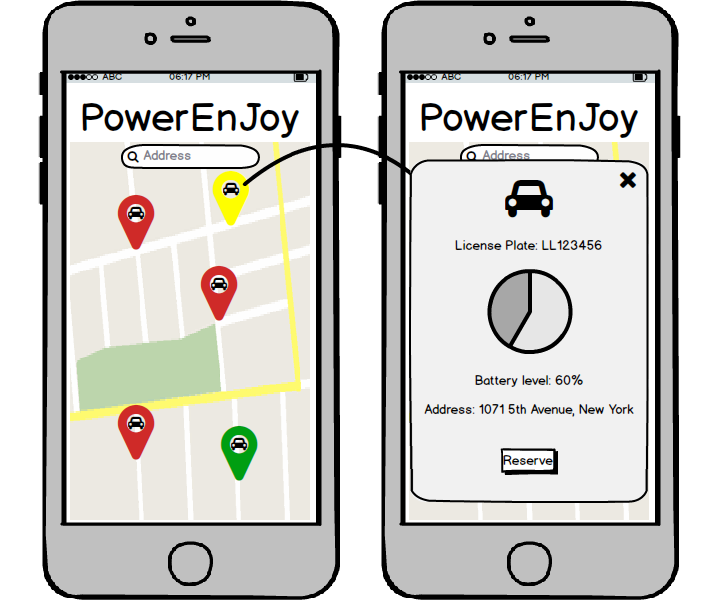
\includegraphics[width=\textwidth]{mockup/MobileSearch.png}
	\caption{Concept for the mobile search page.}
\end{figure}

\subsubsubsection{Use case description and sequence diagram}

\begin{table}[H]
	\begin{center}
		\begin{tabular}{| l | p{0.6\textwidth} |}
			\hline
			Actor & Driver \\
			\hline
			Goal & G1.1
			\\
			\hline
			Input condition & The driver is already logged and chooses to reserve a car.  \\
			\hline
			Event Flow & \begin{enumerate}
				\item The driver opens the home page and search an available car.
				\item Once chosen, the driver clicks on "Reserve".
			\end{enumerate}
			\\
			\hline
			Output condition & The system notifies the driver that he/she succesfully reserved the chosen car \\
			\hline
			
			Exception &  \begin{itemize}
				\item Some exceptions are handled by notifying the driver of the problem through a dynamic message box.				
				The requirements that generate these kind of exceptions are:
				\ref{f-expired},    %The driving license is expired.
				\ref{f-regular}.    %Status of payments is not regular.			
				\item No car is available in the driver's area.
				\end{itemize}
			\\
			\hline
		\end{tabular}
	\end{center}
\end{table}

\begin{figure}[H]
	\begin{center}
		\centering
		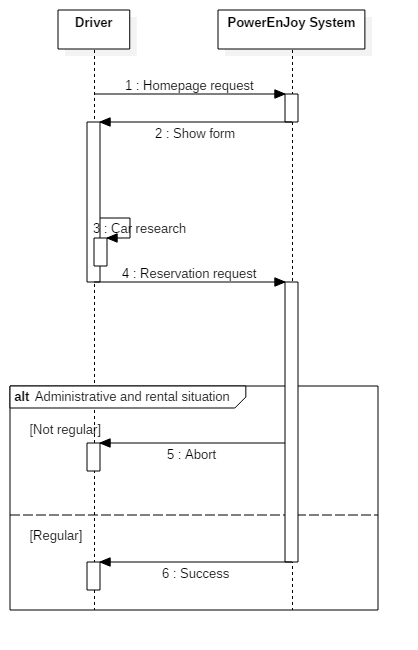
\includegraphics[height=0.9\textheight, keepaspectratio]{sequence_diagram/SearchReservation.png}
		\caption{Sequence diagram of search and reservation process.}
	\end{center}
\end{figure}

\subsubsubsection{Associated functional requirements}

Interactions between system and driver occur through car or mobile applications.

\begin{enumerate}
	\item The driver must be logged into the system in order to search and reserve a car.
	\item The system must show the driver a map of the area, within a 1km range from him/her or from a given address, with the available cars.
	\item The system must provide more informations about an available car. These informations are:
		\begin{itemize}
			\item license plate
			\item address
			\item battery level
		\end{itemize}
	\item In order to reserve a car the driver's driving license mustn't be expired. \label{f-expired}
	\item In order to reserve a car the driver's status of payments must be regular. \label{f-regular}
	\item The system must prevent the driver from reserving more than one car at time.
	\item The system must prevent the driver from reserving a car already reserved, or in use by another driver.
	\item The system must prevent the driver from reserving an "Out\_of\_service" car.
	\item After a reservation is completed, the system automatically tags the reserved car as "Reserved".
	\item After a reservation is completed, the system automatically redirects the driver to the reservation page completed by with the reservation informations.
\end{enumerate}

\subsubsection{Car usage}

\subsubsubsection{Purpose}
The driver can use the car after he/she reserved it.

When the driver is nearby the reserved car he/she can click the button "I'm nearby" on the mobile reservation page and the system will check the GPS signal of both the car and the driver's mobile phone, to assess if they are within a 25 meters range. If they are within that range, the system will unlock the car and the driver can enter it. This operation is available only through the mobile application.

As soon as the engine ignites, the system starts charging the driver for a given amount of money per minute; the driver is notified of the current charges through a screen on the car.

\subsubsubsection{Scenario 1}
Bob has already reserved a car and he is going to pick it up. He is about 50 meters from the car and he clicks the button "I'm nearby" on the mobile application. The system checks the GPS signal of both the car and Bob's mobile phone, and doesn't unlock the car notifying Bob that he's too far from the car.

Once Bob is in front of the car he clicks again on "I'm nearby", the system unlocks the car and he can finally enter.

Bob starts the car and the system notifies him about his current charges through the car application. He can start his ride.

\begin{figure}[H]
	\centering
	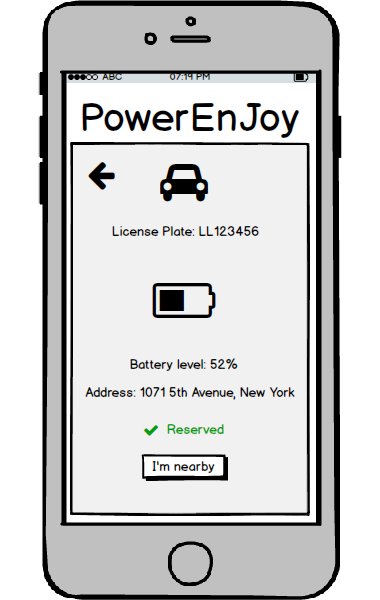
\includegraphics[height=20cm]{mockup/MobileUnlock.png}
	\caption{Concept for the mobile car reservation page.}
\end{figure}

\begin{figure}[H]
	\centering
	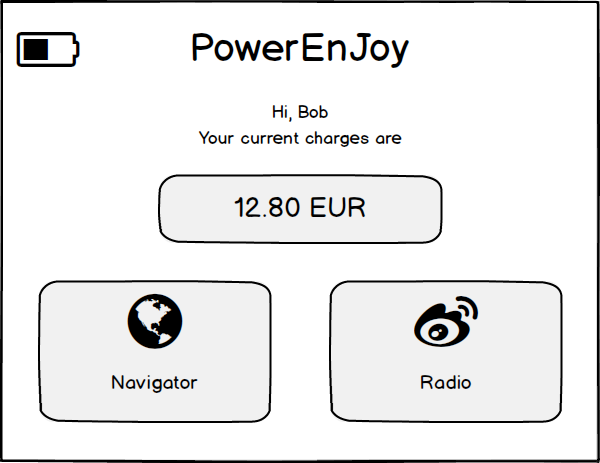
\includegraphics[width=\textwidth]{mockup/VehicleApplication.png}
	\caption{Concept for the car application.}
\end{figure}

\begin{table}[H]
	\begin{center}
		\begin{tabular}{| l | p{0.6\textwidth} |}
			\hline
			Actor & Driver \\
			\hline
			Goal & G1.2
			\\
			\hline
			Input condition & The driver has already reserved a car and he/she is going to pick it up.  \\
			\hline
			Event Flow & \begin{enumerate}
				\item The driver is within 25 meters from the car.
				\item The driver opens the reservation mobile page, through a button of the homepage, and clicks on "I'm nearby".
				\item The system unlocks the car.
				\item The driver enters and starts the car. 
			\end{enumerate}
			\\
			\hline
			Output condition & The driver starts his/her ride and the system keeps notifying him/her about his/her current charges. \\
			\hline
			
			Exception &  \begin{itemize}
				\item Some exceptions are handled by notifying the driver of the problem through a dynamic message box.				
				The requirements that generate these kind of exceptions are:
				\ref{f-reservationcanc},    %It passed more than one hour from the reservation
				\ref{f-nearby}.    %The driver isn't nearby.		
				\item GPS signal of the driver's mobile phone is not available.
				\item GPS signal of the car is not available.		
			\end{itemize}
			\\
			\hline
		\end{tabular}
	\end{center}
\end{table}

\begin{figure}[H]
	\begin{center}
		\centering
		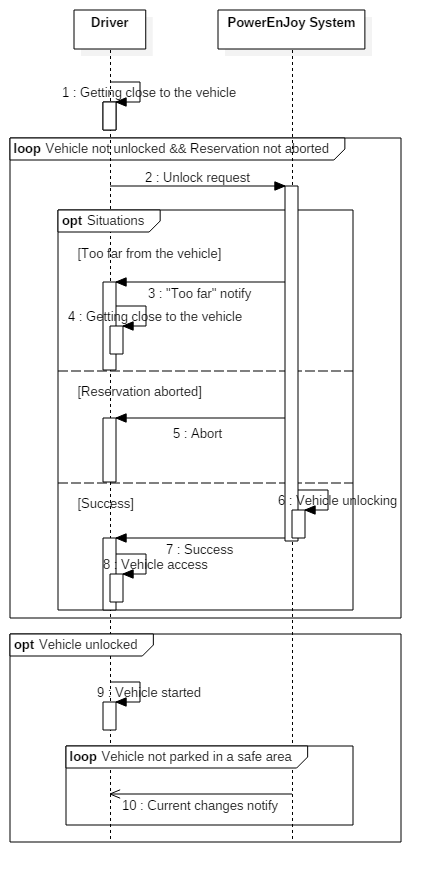
\includegraphics[height=0.9\textheight, keepaspectratio]{sequence_diagram/Unlock.png}
		\caption{Sequence diagram of the car usage process.}
	\end{center}
\end{figure}

\subsubsubsection{Associated functional requirements}

\begin{enumerate}
	\item The driver can only use the mobile application to unlock the car. 
	\item From the reservation to the unlocking of the car must not pass more than one hours. Otherwise the system will tag again the car as "Available". The driver is notified about the end of the rental operation.\label{f-reservationcanc}
	\item The system checks the GPS signal of both the car and driver's mobile phone, to assess if they are within a 25 meters range. If they are within that range, the system will unlock the car. \label{f-nearby}
	\item The driver must enter in the car to start it.
	\item The system will start charging the driver once he/she starts the car.
	\item Once the car is unlocked, the system tags it as "In\_use".
	\item The car application must notify the driver about current charging.	
\end{enumerate}

\subsubsection{Car parking}

\subsubsubsection{Purpose}

Once the driver has finished using the car he/she should be able to park it in safe area provided by the system. These areas are displayed by the navigator car application.

After parking the car, the driver can exit from it. The system will lock the car and automatically charges the driver on the credit card indicated during the registration.

If a driver brought other people with him/her, he/she will get a 10\% discount on the final charge.

\subsubsubsection{Scenario 1}

Bob is almost at his important meeting. The GPS navigator application shows several parking areas and Bob chooses one of them to park his car. He checks if there's at least one available parking spot and he finds one. Once he turns off the car and gets out, the system stops charging him and he can finally enjoy his evening.

\begin{figure}[H]
	\centering
	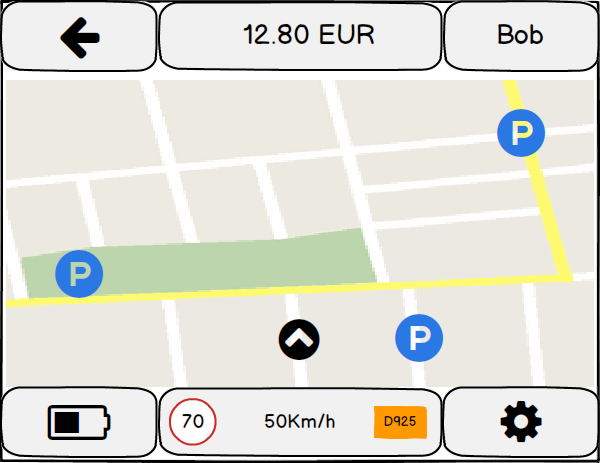
\includegraphics[width=\textwidth]{mockup/VehicleApplicationNavigator.png}
	\caption{Concept for the car application.}
\end{figure}

\begin{table}[H]
	\begin{center}
		\begin{tabular}{| l | p{0.6\textwidth} |}
			\hline
			Actor & Driver with or without guests (passengers) \\
			\hline
			Goals & G1.3, G3
			\\
			\hline
			Input condition & The driver is using the reserved car and wants to park it nearby his/her destination. He/she could be accompanied by some passengers. \\
			\hline
			Event Flow & \begin{enumerate}
				\item The driver finds a parking spot via the car application.
				\item The driver parks the car in an available spot of a safe area.
				\item The driver turns off the car and gets out. If he/she is accompanied by someone, they get out too.
				\item The system checks if the car can be locked and if discounts are applicable. 
			\end{enumerate}
			\\
			\hline
			Output condition & The system locks the car, directly charges the driver via the payment method that he/she indicated during the registration process and notifies him/her that the rental has ended.\\
			\hline
			
			Exception &  \begin{itemize}
				\item The driver has an accident.
				\item The car battery completly run out.	
				\item There's no parking spots available in a nearby safe areas.	
			\end{itemize}
			\\
			\hline
		\end{tabular}
	\end{center}
\end{table}

\begin{figure}[H]
	\begin{center}
		\centering
		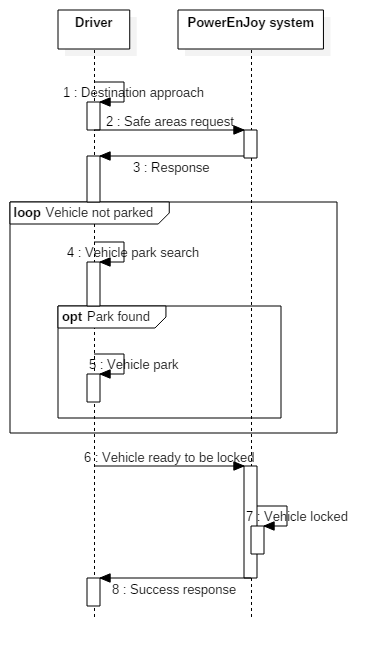
\includegraphics[height=0.9\textheight, keepaspectratio]{sequence_diagram/Park.png}
		\caption{Sequence diagram of the car parking process.}
	\end{center}
\end{figure}

\subsubsubsection{Associated functional requirements}

\begin{enumerate}
	\item The driver must park his/her car in a safe area.
	\item The driver must get out from the car remembering to close all doors and to roll up all windows of the car, otherwise the system won't stop charging him/her, and after 5 minutes will send him/her a sms notification to remember him/her that the rental operation can't be ended correctly.
	After 30 minutes the system tags the car as "Out\_of\_service" and it will apply a fee of 20 euros to the driver.
	\item Once the car is locked, the system must directly charge the driver via the previosly indicate payment method.
	\item Once the car is locked, the system must send a message to notify the driver about rental costs. The rental is now concluded. The reservation page will be cleared and closed by the system.
	\item Once the car is locked, the system checks its conditions. If battery power is lower  than 25\% or a component of it is not working correctly, the system must tag the car as "Out\_of\_service". Otherwise the system tags the car as "Available".
	\item Other requirements for G3 only are:
	\begin{enumerate}
		\item car's sensors must detect correctly the number of passengers.
		\item if the driver is accompanied by at least one passenger during the whole ride, the system will apply him/her a direct discount of 10\%, otherwise there won't be any discount.
	\end{enumerate}
\end{enumerate}

\subsubsection{Service discounts and fees}

\subsubsubsection{Purpose}
During the rental of a car, the driver can be rewarded with discounts or punished with fines.
For instance, if a driver leaves a car with more than 50\% of battery charge, the system applies a discount of 20\% on the last ride.

\subsubsubsection{Scenario 1}

Bob is going too fast because he is late for his important meeting. He commits a serious infraction and gets a speeding ticket. The system pays his fine and directly charges him the same amount of the fine plus an addictional fee of 10 euros. Bob is not happy.

\subsubsubsection{Associated functional requirements}

Requirements for G4 are the following:

\begin{enumerate}
	\item Discounts must be applied one at time on total rental price excluding any fee or fine. The total rental price is updated everytime a discount is applied.
	\item Fines or fees are applied after any discount.
	\item If a driver doesn't pick up a reserved car within 1 hour, the system applies a fine of 1 euro.
	\item If a driver gets a fine, the system pays his/her fine and directly charges him/her by the same amount of the fine plus an addictional fee of 10 euros.
	\item If a driver leaves a car with more than 50\% of battery charge, the system applies a discount of 20\% on the last ride.
\end{enumerate}

\subsection{Performance Requirements}

\begin{enumerate}
	\item The system must support at least 1000 connected driver at time.
	\item 95\% of requests must be processed in less than 5 s.
	\item 100\% of requests must be processed in less than 10 s.
	\item There is no limit on the total number of registered drivers.
\end{enumerate}

\subsection{Alloy}

\lstset{
	language=alloy,
	numbers=left,
	numberstyle=\tiny,
	stepnumber=2,
	tabsize=4,
	keywordstyle=\color{alloy-keyword}\bfseries,
	commentstyle=\color{alloy-comment},
	stringstyle=\color{alloy-string},
	basicstyle=\small\fontfamily{pcr}\selectfont, % Courier font family
}

% Includes the Alloy model file.
\lstinputlisting{alloy/PowerEnJoy.als}
	
	\include{scenario}
	
	\include{uml}
	
	% alloy.sty
% Alloy mode for the LaTeX listings package.
% This is public domain

\lstdefinelanguage{alloy}{
  keywords={%
      assert, pred, all, no, lone, one, some, check, run,
      but, let, implies, not, iff, in, and, or, set, sig, Int, int,
      if, then, else, exactly, disj, fact, fun, module, abstract,
      extends, open, none, univ, iden, seq,
  },
  literate=%
    {:}{$\colon$}1
    {|}{$\bullet$}1
    {==}{$=$}1
    {=}{$=$}1
    {!=}{$\neq$}1
    {&&}{$\land$}1
    {||}{$\lor$}1
    {<=}{$\le$}1
    {>=}{$\ge$}1
    {all}{$\forall$}1
    {exists}{$\exists$}1
    {!in}{$\not\in$}1
    {\\in}{$\in$}1
    {=>}{$\implies$}2
    % the following isn't actually Alloy, but it gives the option to produce nicer latex
    {|=>}{$\Rightarrow$}2
    {<=set}{$\subseteq$}1
    {+set}{$\cup$}1
    {*set}{$\cap$}1
    {==>}{$\Longrightarrow$}3
    {<==>}{$\Longleftrightarrow$}4
    {...}{$\ldots$}1
    {\\hl}{$\hline$}1
    {\\alpha}{$\alpha$}1
    {\\beta}{$\beta$}1
    {\\gamma}{$\gamma$}1
    {\\delta}{$\delta$}1
    {\\epsilon}{$\epsilon$}1
    {\\zeta}{$\zeta$}1
    {\\eta}{$\eta$}1
    {\\theta}{$\theta$}1
    {\\iota}{$\iota$}1
    {\\kappa}{$\kappa$}1
    {\\lambda}{$\lambda$}1
    {\\mu}{$\mu$}1
    {\\nu}{$\nu$}1
    {\\xi}{$\xi$}1
    {\\pi}{$\pi$}1
    {\\rho}{$\rho$}1
    {\\sigma}{$\sigma$}1
    {\\tau}{$\tau$}1
    {\\upsilon}{$\upsilon$}1
    {\\phi}{$\phi$}1
    {\\chi}{$\chi$}1
    {\\psi}{$\psi$}1
    {\\omega}{$\omega$}1
    {\\Gamma}{$\Gamma$}1
    {\\Delta}{$\Delta$}1
    {\\Theta}{$\Theta$}1
    {\\Lambda}{$\Lambda$}1
    {\\Xi}{$\Xi$}1
    {\\Pi}{$\Pi$}1
    {\\Sigma}{$\Sigma$}1
    {\\Upsilon}{$\Upsilon$}1
    {\\Phi}{$\Phi$}1
    {\\Psi}{$\Psi$}1
    {\\Omega}{$\Omega$}1
    {\\EOF}{\;}1
    ,
  sensitive=true,  % case sensitive
  morecomment=[l]//,%
  morecomment=[l]{--},%
  morecomment=[s]{/*}{*/},%
  morestring=[b]",
  numbers=none,
  firstnumber=1,
  numberstyle=\tiny,
  stepnumber=2,
  basicstyle=\scriptsize\ttfamily,
  commentstyle=\itshape,
  keywordstyle=\bfseries,
  ndkeywordstyle=\bfseries,
}

% inline
\def\A{%
    \lstinline[language=alloy,basicstyle=\ttfamily,columns=fixed]}

% paragraph
\lstnewenvironment{alloy}[1][]{%
  \lstset{language=alloy,
    floatplacement={tbp},captionpos=b,
    xleftmargin=8pt,xrightmargin=8pt,basicstyle=\ttfamily,#1}}{}

% paragraph from file
\newcommand{\alloyfile}[1]{
  \lstinputlisting[language=alloy,%
    frame=lines,xleftmargin=8pt,xrightmargin=8pt,basicstyle=\ttfamily,columns=fixed]{#1}
}
	
	\section{Appendix}
\subsection{Used tools}
To create the RASD we used the following tools:
\begin{itemize}
	\item \textbf{MikTex} \\ JUnit is a simple framework to write repeatable tests. It is an instance of the xUnit architecture for unit testing frameworks.
 \\ \url{http://junit.org/junit4/} 
	\item \textbf{TexStudio}\\ OpenSource cross-platform LaTeX editor we used to write the RASD. \\ \url{http://texstudio.sourceforge.net/} 
	\item \textbf{StarUML}\\ UML modelling tool we used to build the graphs\\ \url{http://staruml.io/} 
	\item \textbf{Balsamiq}\\ The mockup builder we used to design the mockups. \\ \url{https://balsamiq.com/} 
	\item \textbf{Alloy analyzer 4}\\ used to build  strong and substantial models \\ \url{ http://alloy.mit.edu/alloy/}
	\item \textbf{GitHub desktop}\\ Desktop application of the web-based Git repository hosting service. Used to collaborate in the team and to have a track of the changes.  \\ \url{https://desktop.github.com/} 
\end{itemize}


\subsection{Hours of work}
This is the time spent redacting the RASD
\begin{itemize}
	\item {Lorenzo Binosi} - 80 hours
\end{itemize}

\begin{thebibliography}{1}	
	\bibitem{se-project-rules}
	Software Engineering 2 Project, AA 2016/2017 - \emph{Project goal, schedule and rules}
	
	\bibitem{se-assignment}
	Software Engineering 2 Project, AA 2016/2017 - \emph{Assignments 1}
	
	\bibitem{ieee-830-1198}
	IEEE Standard 830-1998: \emph{IEEE Recommended Practice for Software Requirements Specifications}
	
	\bibitem{w3c-html5}
	W3C, \emph{HTML5 - W3C Recommendation 28 October 2014}, \url{http://www.w3.org/TR/html5/}.
	
	\bibitem{w3c-css}
	W3C, \emph{Cascading Style Sheets Level 2 Revision 1 (CSS 2.1) Specification}, \url{http://www.w3.org/TR/CSS21/}
	
	\bibitem{apple-ios-hig}
	Apple, \emph{iOS Human Interface Guidelines}, \url{https://developer.apple.com/library/ios/documentation/UserExperience/Conceptual/MobileHIG/}
	
	\bibitem{google-android-hig}
	Google, \emph{Android Developers - Design}, \url{https://developer.android.com/design/index.html}
\end{thebibliography}
	
\end{document}